\chapter{Ala ma kota}

ĄĆĘŁŃÓŚŹŻ ąćęłńóśźż\footnote{Przykład użycia polskich znaków diakrytycznych oraz przypisu w miejscu}. \lipsum[1]

\section{Odniesienie do pozycji z literatury (strona WWW)}

% Odniesienie do rysunku i cytowanie dokumentu. Dokumenty są definiowane w pliku literatura.bib
Reszta dokumentacji znajduje się w \cite{docker_compose_reference}. \lipsum[3]

\section{Odniesienie do książki}

Jak pisze Harel w \cite{harel_rzecz_2008}: \lipsum[7]

\section{Rysunek}

% Rysunek
\begin{figure}
\centering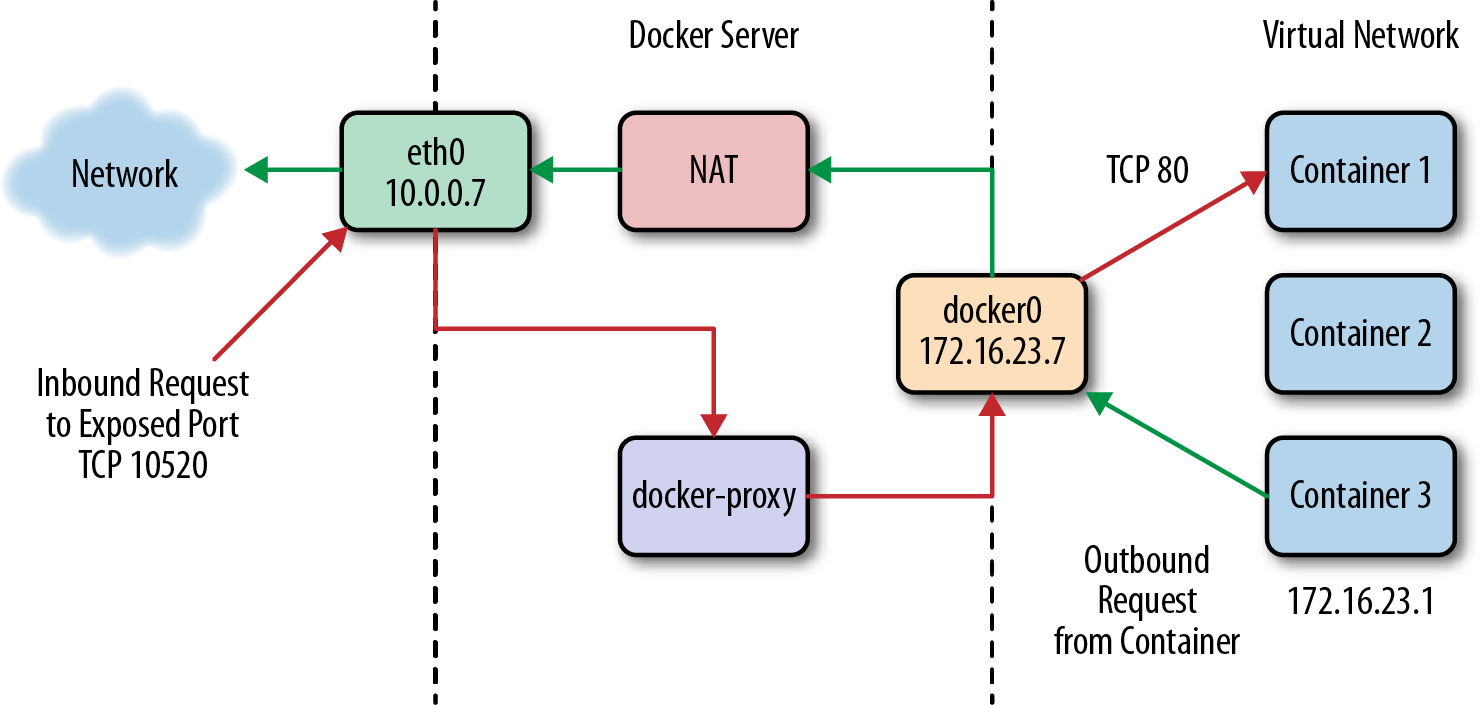
\includegraphics[width=.6\textwidth]{img/swarm-network}
\caption{Docker ma sieć \cite{docker_compose_reference}.}  \label{rys:network}% Źródło rysunku i etykieta przez którą odwołujemy się do rysunku.
\end{figure}

Jak widać na rys. \ref{rys:network} Docker ma wewnętrzną sieć. \lipsum[1]


\subsection{Rysunek z kotem}

Jak widać na rys.\ref{rysunek:kot} Ala ma kota. \lipsum[9-10] 

\begin{figure}[h!]
\centering
\includegraphics[width=.4\textwidth]{img/kotek}
\caption{Ala ma kota (opr.wł).}\label{rysunek:kot}
\end{figure}

\subsection{Tabela}

Co uwzględniono w tabeli \ref{tabela:coktoma}. \lipsum[13-15] 

% Tabela. Nazwa tabeli u góry.
\begin{table}[h!]
\centering\caption{Co kto ma \cite{harel_rzecz_2008} (patrz też dodatek~\ref{Dod1}) \label{tabela:coktoma}}
\begin{tabular}{|l|l|l|}% wyrównanie kolumn tabeli -> l c r - do lewej, środka, do prawej
\hline
Ala & ma & kota \\
\hline
Ola & ma & psa \\
\hline
Ula & ma & małpę\\
\hline
\end{tabular}
\end{table}

\lipsum[19-20] Warto wspomnieć, że w \cite{aizawa_groundwater_2009} rzecz przedstawiona jest zupełnie inaczej. Poniższy wzór:

\begin{equation}
\sum_{i=1}^{\infty}a_i
\label{eq:mojWzor}
\end{equation}

Wzór \ref{eq:mojWzor} wskazuje że dowód podany w \cite{kaleta_experimental_2005} może zostać podważony. \lipsum[9]

\section{Kod źródłowy}

% lub {java} albo {bash} albo {text}
\begin{listing}[h!]
\begin{minted}{c} 
int main()
{
   int a=2*3;
   printf("**Ala ma kota\n**");
   while(!I2C_CheckEvent(I2C1, I2C_EVENT_MASTER_MODE_SELECT)); /* EV5 */
   return 0;
}
\end{minted}
\caption{Przykładowy algorytm w języku C (opr. wł.)} \label{listing:moj}
\end{listing}

W moim kodzie \ref{listing:moj} zrobiłem coś wspaniałego. \lipsum[4]

\begin{table}[h]
	\begin{tabularx}{\textwidth}{|>{\setlength\hsize{1.4\hsize}\setlength\linewidth{\hsize}}X|>{\setlength\hsize{.9\hsize}\setlength\linewidth{\hsize}}X|>{\setlength\hsize{.7\hsize}\setlength\linewidth{\hsize}}X|}
		\hline
		\multicolumn{3}{|c|}{Classification of the criticel point $(0,0)$ of $x'=Ax,|\mathbf{A}|\not=0$.}\\
		\hline
		Types & Type of Critical Point & Stability \\
		\hline
		1. Real unequal eigenvalues of same sign
		\begin{itemize}
			\item $\lambda_1 > \lambda_2 > 0$
			\item $\lambda_1 < \lambda_2 < 0$
		\end{itemize} &
		\vphantom{1. Real unequal eigenvalues of same sign}
		\begin{itemize}
			\item Improper Node/Node
			\item Improper Node/Node
		\end{itemize} &
		\vphantom{1. Real unequal eigenvalues of same sign}
		\begin{itemize}
			\item Unstable
			\item Asym. Stable
		\end{itemize}\\
		\hline
		2. Real unequal eigenvalues of opposite sign
		\begin{itemize}
			\item $\lambda_2 < 0 >\lambda_1$
		\end{itemize} &
		\vphantom{2. Real unequal eigenvalues of opposite sign}
		\begin{itemize}
			\item Saddle Point
		\end{itemize} &
		\vphantom{2. Real unequal eigenvalues of opposite sign}
		\begin{itemize}
			\item Unstable
		\end{itemize}\\
		\hline
		3. Equal eigenvalues \newline Subtype 1: Two Independent vectors
		\begin{itemize}
			\item $\lambda_1 = \lambda_2 > 0$
			\item $\lambda_1 = \lambda_2 < 0$
		\end{itemize} &
		\vphantom{3. Equal eigenvalues} \vphantom{ Subtype 1: Two Independent vectors}
		\begin{itemize}
			\item Proper Node
			\item Proper Node
		\end{itemize} &
		\vphantom{3. Equal eigenvalues} \vphantom{ Subtype 1: Two Independent vectors}
		\begin{itemize}
			\item Unstable
			\item Asym. Stable
		\end{itemize}\\
		\hline
	\end{tabularx}
\end{table}
\thispagestyle{normal}